% Copyright 2007 by Till Tantau
%
% This file may be distributed and/or modified
%
% 1. under the LaTeX Project Public License and/or
% 2. under the GNU Public License.
%
% See the file doc/licenses/LICENSE for more details.


\lecture[22]{Correlation}{lecture-text}

\subtitle{and the correlation coefficient}

\date{21 April 2015}

% pp. 480-492




\begin{document}

\begin{frame}
  \maketitle
\end{frame}



\begin{frame}{Relationships so far}
  \begin{enumerate}
    \item To answer the question ``is there a relationship between $X$ and $Y$'',
      so far we can answer if
    \item $X$ and $Y$ are categorical (probability of assignment for $X$ depends on $Y$); $\chi^2$ test
    \item $X$ is categorical and $Y$ is quantitative (mean of $Y$ depends on $X$); one-way ANOVA
  \end{enumerate}
\end{frame}

\begin{frame}\frametitle<presentation>{Outline}
  \tableofcontents
\end{frame}


\section{Scatterplots}

%%%%%%
\begin{frame}{Example:}

  \textit{Toxoplasma gondii} infection rates and measures of aggregate neuroticism in 31 countries:

  \begin{center}
    \only<1>{
    \scriptsize
\begin{tabular}{lrr|lrr}
  \hline
  country & prevalence (\%) & N18 &
  country & prevalence (\%) & N18 \\ 
  \hline
Argentina    &  52.70  &  51.30   & Japan        &  12.30  &  50.70  \\
Australia    &  28.00  &  48.60   & Netherlands  &  24.50  &  48.60  \\
Austria      &  36.00  &  48.30   & Norway       &  8.60   &  47.40  \\
Belgium      &  46.80  &  49.60   & Peru         &  32.90  &  48.50  \\
Brazil       &  66.90  &  53.70   & Poland       &  46.50  &  50.70  \\
China        &  24.30  &  53.10   & SouthKorea   &  4.30   &  48.40  \\
Croatia      &  37.40  &  49.30   & Slovenia     &  30.90  &  50.60  \\
CzechRep     &  26.60  &  51.40   & Spain        &  22.70  &  49.70  \\
Denmark      &  22.00  &  50.30   & Sweden       &  12.50  &  46.30  \\
Ethiopia     &  16.40  &  48.80   & Switzerland  &  36.70  &  47.50  \\
France       &  45.00  &  52.70   & Thailand     &  11.20  &  48.90  \\
Germany      &  42.70  &  48.10   & Turkey       &  46.80  &  51.40  \\
Hungary      &  58.90  &  53.80   & UK           &  6.60   &  50.10  \\
Indonesia    &  46.20  &  50.00   & USA          &  12.30  &  48.10  \\
Ireland      &  25.00  &  50.10   & Yugoslavia   &  66.80  &  51.10  \\
Italy        &  32.60  &  52.60   &  & & \\
   \hline
\end{tabular}
\figcaption{Lafferty 2006, ``Can the common brain parasite, \textit{Toxoplasma gondii}, influence human culture? ''}
    }
    \only<2>{
    \includegraphicscopyright{ex24-toxo}{Lafferty 2006, ``Can the common brain parasite, \textit{Toxoplasma gondii}, influence human culture? ''}
    }
    \only<3>{
    \includegraphicscopyright{ex24-toxo-line}{Lafferty 2006, ``Can the common brain parasite, \textit{Toxoplasma gondii}, influence human culture? ''}
    }
  \end{center}

\end{frame}

\section{Correlation}

%%%%%%
\begin{frame}{The idea of correlation}

  The goal is to describe
  \begin{itemize}
    \item the strength of the relationship between two variables
    \item in a \alert{scale--free} way.
  \end{itemize}
  In other words, it shouldn't depend on the units used to measure $X$ and $Y$.

    \vspace{2em}

    First step: \alert{transform} $X$ and$Y$ to $z$-scores: \\
    \uncover<2>{
    \centering
    \includegraphicscopyright[height=1.5in]{ex24-toxo-sdized}{}
    }

\end{frame}

%%%%%%
\begin{frame}{The correlation coefficent}

  One scale-free measure of the strength of a relationship is (Pearson's product-moment) \alert{correlation coefficient}:
  \begin{enumerate}
    \item Subtract the means from each variable ($x_i-\bar x$ and $y_i-\bar y$)
    \item Divide by the standard deviations ($z_x=(x_i-\bar x)/s_x$ and $z_y=(y_i-\bar y)/s_y$)
    \item Add their products and divide by the degrees of freedom ($\sum_i z_x z_y / (n-1)$)
  \end{enumerate}
  \[
    r = \frac{1}{n-1} \sum_{i=1}^n \left(\frac{x_i-\bar x}{s_x}\right)\left(\frac{y_i-\bar y}{s_y}\right)
  \]

\end{frame}

%%%%%%
\begin{frame}{What does it mean?}
  \begin{itemize}
    \item $r$ is between -1 and 1
    \item $|r|=1$ means perfect \alert{linear} relationship
    \item $r=0$ means no linear relationship
    \item larger $|r|$ means stronger linear relationship
    \item $r<0$ means inverse relationship
  \end{itemize}

  \begin{center}
    \includegraphicscopyright[width=\textwidth]{506px-Correlation_examples2.png}{Wikimedia Commons}
  \end{center}

\end{frame}

%%%%%%
\begin{frame}{Example}
  \textit{Toxoplasma gondii} infection rates and measures of aggregate neuroticism in 31 countries:
    \includegraphicscopyright{ex24-toxo}{Lafferty 2006, ``Can the common brain parasite, \textit{Toxoplasma gondii}, influence human culture? ''}

    % Relationship:
    % \[ \text{(neuroticism)} \approx 48.09 + 0.06 \times \text{(Toxoplasma percent)} \]
    correlation coefficient:
    \[ r = 0.54 .  \]

\end{frame}

\section{What is $r$?}

%%%%%%
\begin{frame}{What is the purpose of $r$?}

  \structure{Summary statistic:} a numerical quantity computed to summarize some aspect of the data.

    \vspace{1em}

  \structure{Parameter estimate:} a particular sort of summary statistic, designed to estimate some population parameter (when applied to a random sample).

    \vspace{2em}

  \structure{Examples:} ($\bar y$)
  \begin{enumerate}
    \item The average height of the 50 people at my family reunion was 5'8". \alert{\it (summary statistic)}
    \item The average height of a random sample of 50 USC undergraduates was 5'8". \alert{\it (parameter estimate)}
  \end{enumerate}

\end{frame}

%%%%%%
\begin{frame}{Things $r$ might estimate}

  Two sorts of parameters we might be estimating:
  \begin{enumerate}
    \item The population correlation between $X$ and $Y$ \\
      -- data are independently sampled pairs $(X,Y)$. \\
      \structure{ex:} (shoulder width, forearm length)
    \item The linear mean effect of $X$ on $Y$ \\
      -- data are measurements of $Y$ across values of $X$. \\
      \structure{ex:} (dose, response) 
  \end{enumerate}

    \vspace{2em}

    In the second case noise might be inherent randomness in the response
    (the \alert{mean response} is a linear function of $X$) \\
    or the result of noisy measurement of $Y$ (true relationship is linear; noise is unbiased)

\end{frame}

\section{Hypothesis testing}

%%%%%%
\begin{frame}{A null hypothesis}

  The correlation coefficient mesaures the strength of a linear relationship.
  Usually, the null hypothesis is \alert{no (linear) relationship}, or
  \[ H_0 : r=0 . \]


    \vspace{2em}

    \structure{Examples:}\\
    \vspace{1em}
    $H_0$: There is no linear relationship between Toxoplasma prevalence and neuroticism.\\
    \vspace{1em}
    $H_0$: Son's height is not correlated with father's height.

\end{frame}

%%%%%%
\begin{frame}{A null distribution}

  Under the null hypothesis of no correlation 
  {\small (and Normal sampling distributions, independent paired observations)}
  the distribution of $r$ is related to $t$:
  \[
    t_s = r \sqrt{\frac{n-2}{1-r^2}}
  \]
  is $t$-distributed with $df=n-2$.



\end{frame}

%%%%%%
\begin{frame}{Example: snakes}

  \begin{center}
    \includegraphicscopyright[width=\textwidth]{table-12-2-2.png}{SWS, Table 12.2.2}
  \end{center}

\end{frame}

\begin{frame}
  \begin{center}
    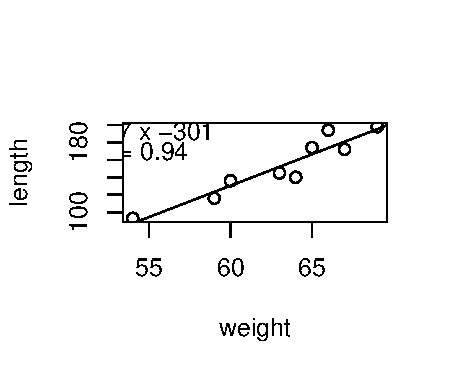
\includegraphics[width=\textwidth]{snakes-cor-ex}
  \end{center}
\end{frame}

\section{Interpreting correlations}

%%%%%%
\begin{frame}{Correlation is not causation}

  \begin{center}
    \includegraphicscopyright[width=.8\textwidth]{xkcd-correlation.png}{xkcd.com/552}
  \figcaption{``Correlation doesn't imply causation, but it does waggle its eyebrows suggestively and gesture furtively while mouthing `look over there'.''}
  \end{center}


    \vspace{2em}

    \structure{Also,} remember that statistical significance \alert{does not imply real-world significance}.


\end{frame}


%%%%%%
\begin{frame}{Example:}


  \textit{Toxoplasma gondii} infection rates and measures of aggregate neuroticism in 31 countries:
  \only<1>{
  \begin{center}
    \includegraphicscopyright{ex24-toxo-line}{Lafferty 2006, ``Can the common brain parasite, \textit{Toxoplasma gondii}, influence human culture? ''}
  \end{center}
  }


  \only<2->{
    \vspace{1em}

    Relationship:
    \[ \text{(neuroticism)} \approx 48.09 + 0.06 \times \text{(Toxoplasma percent)} \]
    correlation coefficient:
    \[ r = 0.54 .  \]
    $t$-statistic:
    \begin{align*} 
      t_s &= 0.54 \sqrt{ \frac{ 31-2 }{ 1 - 0.54^2 } } = 3.484685  \\
      df &= 29 \\
      0.001 &< P < 0.01
    \end{align*} 
    }

    \alert{What can we conclude?}

\end{frame}


% %%%%%%
% \begin{frame}{Example: rats on drugs}
% 
%   Amount of food consumed by 24 rats, randomly given one of three amounts of amphetamine:
%   \begin{center}
%     \only<1>{ \includegraphicscopyright[width=.8\textwidth]{fig-12-1-1.png}{figure 12.1.1} }
%     \only<2>{ \includegraphicscopyright[width=.8\textwidth]{table-12-1-1.png}{table 12.1.1} }
%   \end{center}
% 
% 
% \end{frame}
% % . . . 


\section<article>{Summary}
\section<presentation>*{Summary}

\begin{frame}{Summary}
  \begin{enumerate}
    \item The correlation coefficient 
    \item (a.k.a.\ Pearson's product-moment correlation)
    \item is a scale-free measure of the strength of a linear relationship between two variables,
    \item is computed as the sum of the products of the $z$-scores, divided by $n-1$,
    \item and the significance can be computed with a $t$-test.
  \end{enumerate}
\end{frame}

% homework
\begin{frame}{Homework}
  \begin{center}

    12.2.1

  \vspace{2em}

  12.2.5

  \vspace{2em}

  12.2.6

  \end{center}
\end{frame}


\end{document}





